\chapter{Metriken}
    \section{Vergleich von Bildern}
        \subsection{Mean Squared Error}
            Der Mean Squared Error (MSE) ist eine gängige Metrik zum Messen von Vorhersagen oder Rekonstruktionen.
            Er misst die durchschnittliche quadratische Differenz den tatsächlichen/ originalen Daten und den vorhergesagten/ rekonstruierten Daten.
            Ein niedriger MSE deutet darauf, dass das rekonstruierte oder vorhergesagte $\hat{x}$ nahe am original $x$ liegt.\bigskip
            \begin{center}
                $\text{MSE} = \frac{1}{n} \sum_{i=1}^{n} (x_i - \hat{x}_i)^2$
            \end{center}

            \begin{enumerate}
                \item Vorteile
                \begin{itemize}
                    \item Große Fehler werden durch das Quadrieren stärker bestraft. Dies ist von Vorteil, wenn große Fehler minimiert werden sollen. \cite{mse_builtin}.
                    \item Der MSE ist zudem mathematisch einfach zu berechnen.
                \end{itemize}
                \item Nachteile
                \begin{itemize}
                    \item Der MSE ist empfindlich gegenüber Ausreißern. Er bestraft große Fehler (Ausreißer) unverhältnismäßig stark, da die Fehler quadriert werden. Ein einziger großer Fehler kann den gesamten MSE-Wert erheblich erhöhen, selbst wenn die meisten anderen Fehler gering sind. \cite{mse_builtin}
                    \item             
                    Sowohl der MSE als auch der PSNR sind Metriken, die sich ohne hohen Aufwand
                    implementieren und berechnen lassen. Sie haben jedoch einige Einschränkungen: Der
                    MSE berücksichtigt nicht die Wahrnehmung des menschlichen Auges und kann daher
                    Unterschiede in der visuellen Qualität nicht immer genau erfassen. \cite{mse_psnr_eye}
                \end{itemize}
            \end{enumerate}

\newpage
        \subsection{Peak Signal-to-Noise Ratio}
            Die Peak Signal-to-Noise Ratio (PSNR) ist eine Metrik, mit der sich die Qualität eines rekonstruierten oder komprimierten Bildes im Vergleich zum Original ermitteln lässt.
            Der PSNR misst den sogenannten Rauschpegel zwischen dem Originalbild und dem rekonstruierten Bild.
            Ein hoher PSNR-Wert deutet auf eine bessere Qualität hin, da das Rauschen bzw. die Differenz zum Original geringer ist.
            \cite{psnr, psnr2}
            \begin{center}
                $\text{PSNR} = 10 \cdot \log_{10} \left( \frac{\text{MAX}^2}{\text{MSE}} \right)$
            \end{center}
            \begin{enumerate}
                \item Vorteile
                \begin{itemize}
                    \item Einheitliche Skala in Dezibel lässt sich gut interpretieren.\cite{psnr3}
                    \item Sowie beim MSE hat PSNR eine starke Gewichtung auf große Fehler.
                \end{itemize}
                \item Nachteile
                \begin{itemize}
                    \item Da der PSNR ebenfalls auf dem MSE basiert, erbt er dessen Empfindlichkeit gegenüber Ausreißern, sowie andere Nachteile wie das PSNR nicht die Menschliche Wahrnehmung berücksichtigt.
                    \item PSNR berücksichtigt nicht, wie Menschen Bilder wahrnehmen. Kleinere Details oder Farbabweichungen, die für das menschliche Auge vielleicht weniger auffällig sind, werden im PSNR-Wert genauso stark gewichtet wie wichtige Bilddetails.\cite{mse_psnr_eye}
                \end{itemize}
            \end{enumerate}

\newpage
        \subsection{Structural Similarity Index}
            \cite{ssim_paper}
            Der Structural Similarity Index (SSIM) ist eine weitere Metrik zur Messung der Bildqualität. Im Gegensatz zu PSNR und MSE berücksichtigt SSIM die Wahrnehmung des menschlichen Auges.
            Bilder werden hinsichtlich ihrer Struktur, Helligkeit und Kontrast bewertet.
            
            \begin{center}    
                Die \textbf{Helligkeit $(l)$} \vspace{1mm} lässt sich berechnen durch \\
                $l(x, y) = \frac{2 \mu_x \mu_y + C_1}{\mu_x^2 + \mu_y^2 + C_1}$ \vspace{1mm}\\
                wo $\mu_x$ und $\mu_y$ die Mittelwerte der Pixelintensität von $x$ und $y$ sind.\\
                $C_1 = (K_1 \cdot L)^2$ zur vermeidung von Störungen, $K_1 \approx 0.01$ und
                $L = \max(p), \quad p \in (0, 255) \max$.\\
            \end{center}
            \begin{center}    
                Der \textbf{Kontrast $(c)$} \vspace{1mm} lässt sich berechnen durch \\
                $c(x, y) = \frac{2 \sigma_x \sigma_y + C_2}{\sigma_x^2 + \sigma_y^2 + C_2}$ \vspace{1mm}\\
                $\sigma_x$ und $\sigma_y$ sind die Standardabweichungen der Pixelintensität von $x$ und $y$.\\
                $C_2 = (K_2 \cdot L)^2 \quad \text{mit} \quad K_2 \approx 0.03$
            \end{center}
            \begin{center}    
                Der \textbf{Struktur  $(s)$} \vspace{1mm} lässt sich berechnen durch \\
                $s(x, y) = \frac{\sigma_{xy} + C_3}{\sigma_x \sigma_y + C_3}$ \vspace{1mm}\\
                $\sigma_{xy}$ ist die Kovarianz zwischen $x$ und $y$.\\
                $C_3 = (C_2 / 2)$
            \end{center}
            
            \begin{center}    
                $\text{SSIM}(x, y) = [l(x, y)]^\alpha \cdot [c(x, y)]^\beta \cdot [s(x, y)]^\gamma$
            \end{center}
       
            \begin{enumerate}
                \item Vorteile
                \begin{itemize}
                    \item Die Berücksichtigung der menschlichen Wahrnehmung ist beim SSIM gegeben. SSIM wurde entwickelt, um die wahrgenommene Bildqualität besser durch Helligkeit, Struktur und Kontrast erfassen zu können.
                    \cite{wikipedia_ssim}
                    \item Studien haben ergeben, dass der SSIM eine höhere Korrelation mit der subjektiven menschlichen Wahrnehmung der Bildqualität aufweist als beispielsweise die PSNR Metrik.\cite{wikipedia_ssim}
                \end{itemize}
                \item Nachteile
                \begin{itemize}
                    \item Die Berechnung des SSIM ist wesentlich Komplexer und erfordert mehr Rechenleistung.
                \end{itemize}
            \end{enumerate}    

\newpage
    \section{Vergleich von Bildern mit Labels}
        \subsection{Precision}
            Die Vorhersagen des Modells sollten möglichst präzise sein. Je näher die Präzision (Precision) eines Modells an einem Wert von 1.0 liegt, desto besser.
            Ein Modell das einen Wert \text{„1“} Vorhersagt, dann soll auch wirklich der Wert eine \text{„1“} sein.
            Dies wird mit der Precision gemessen.\newline
            \begin{center}  
                \large$prescicion = \frac{\text{true positives}}{\text{true positives} + \text{false positives}}$\\
            \end{center}
            \underline{Bedeutung}\\
            Wieviel Prozent der vorhergesagten positiven Fälle (\text{„1“}) sind wirklich auf wirklich positiv?

            
        \subsection{Recall}
            Vorhersagen sollen eine hohe Trefferquote haben. Das heißt, dass das Modell alle \text{„1“} Fälle in den
            Daten auch als diese erkennt. Hierfür wird die Metrik Recall verwendet.\newline
            \begin{center}  
                \large$recall = \frac{\text{true positives}}{\text{true positives} + \text{false negatives}}$\\
            \end{center}
            \underline{Bedeutung}\\
            Wieviel Prozent der tatsächlichen positiven Fälle (\text{„1“}) erkennt das Modell?
            
        \subsection{F1}
            Der $F1$ Score sagt aus wie gut ein Modell eine hoher Trefferquote hat jedoch auch gleichzeitig wie Präzise es
            ist. Vorhersagen sollen sowohl eine hohe Trefferquote haben als auch Präzise sein.\newline
            \begin{center} 
                \large$F1 = 2 * \frac{\text{precission} * \text{recall}}{\text{precission} + \text{recall}}$\\
            \end{center}
            
\newpage
    \section{Intersection over Union}
        \cite{iou, iou_paper, iou_2} Der Intersection over Union (IoU) wird zur Bewertung der Leistung von Objekterkennungsmodellen verwendet, indem die vorhergesagte Boundingbox (Begrenzungsbox) mit der tatsächlichen (Ground-Truth-Boundingbox) verglichen wird.
        Die IoU ist eine Metrik, mit der jeder Algorithmus bewertet werden kann, der vorhergesagte Boundingboxen als Ausgabe liefert.

        Um IoU zur Bewertung eines beliebigen Objekterkennungsmodells anzuwenden, benötigen man:

        \begin{itemize}
            \item Die Ground-Truth-Boundingboxen sind markierte Boundingboxen aus dem Originaldatensatz (Labeldatensatz), die die genaue Position des Objekts im Bild angeben.
            \item Die Boundingboxen, die vom Modell vorhergesagt werden.
        \end{itemize}
        Solange diese beiden Sätze von Boundingboxen vorliegen, lässt sich der IoU messen.

        \begin{figure}[!htb]
            \centering
            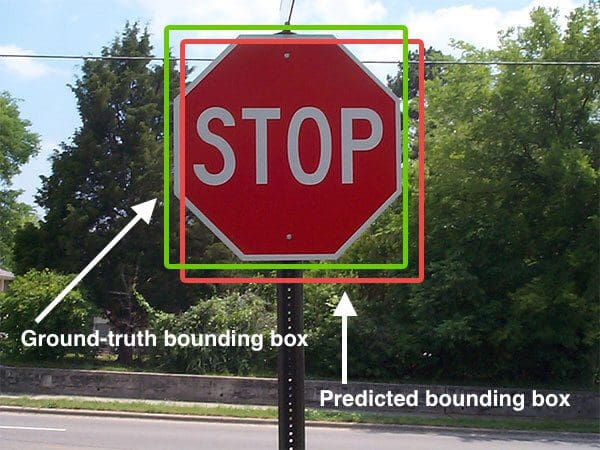
\includegraphics[scale=0.49]{pictures/iou_stop_sign.jpg}
            \caption{Die vorhergesagte Boundingboxe wird in Rot dargestellt, während die Ground-Truth-Boundingboxe in Grün dargestellt wird.\cite{iou}}
        \end{figure}

\newpage
        \cite{iou}
        Die IoU zwischen der vorhergesagten Boundingbox und der Ground-Truth-Boundingbox lässt sich einfach berechnen:
        Die Fläche der Schnittmenge wird durch die Fläche der Vereinigung der beiden Boundingboxen dividiert.
        
        \begin{center}  
            $Area = x2 y2 - x1 y1$\\
            wobei $x1y1$ obere linke Ecke und $x2y2$ untere rechte Ecke\\ \bigskip
            \large$IoU = \frac{Area_{Ground-Truth} \cap Area_{predicted}}{Area_{Ground-Truth} \cup Area_{predicted}}$
        \end{center}

        \begin{figure}[!htb]
            \centering
            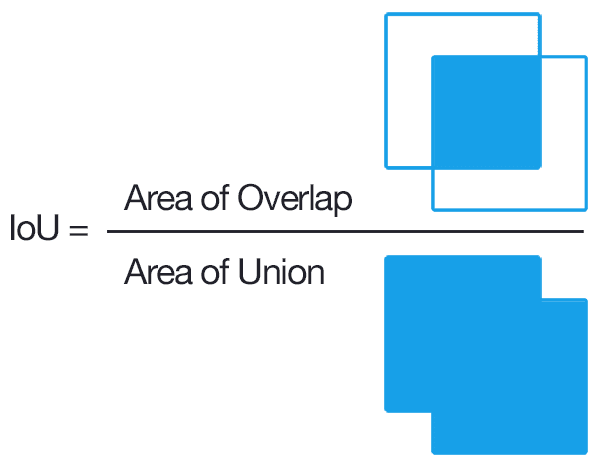
\includegraphics[scale=0.49]{pictures/iou_equation.png}
            \caption{Berechnung des IoU als Grafik.\cite{iou}}
        \end{figure}

        Bei der Verwendung von IoU als Bewertungsmetrik muss ein Schwellenwert (Threshold) für die Genauigkeit festgelegt werden, der in der Regel bei 0,5 liegt. Werte darüber werden als gut bewertet, während Werte darunter als unbrauchbar gelten.\cite{iou_paper, iou_2}
